\documentclass[10pt,a4paper]{article}
\usepackage[left=2cm,right=2cm,top=2cm,bottom=2cm]{geometry}
\usepackage[T1]{fontenc}
\usepackage{lmodern}
\usepackage[spanish,es-tabla,es-noquoting]{babel}
\usepackage[dvipsnames]{xcolor}
\usepackage[fleqn]{mathtools}
\usepackage{booktabs}
\usepackage{amsmath}
\usepackage{latexsym}
\usepackage{graphicx}
\usepackage{nccmath}
\usepackage{multicol}
\usepackage{listings}
\usepackage{color}
\usepackage{float}
\usepackage{csquotes}
\usepackage[backend=biber,style=numeric,sorting=none]{biblatex}
\addbibresource{referencias.bib}

\definecolor{colorIPN}{rgb}{0.5, 0.0,0.13}
\definecolor{colorESCOM}{rgb}{0.0, 0.5,1.0}
\graphicspath{ {imagenes/} }

\begin{document}
%#########################################################
\begin{titlepage}
	\centering
	{ \huge \bfseries \color{colorIPN}{Instituto Politécnico Nacional} \par}
	{ \Large \bfseries  \color{colorESCOM}{Escuela Superior de Cómputo} \par }
	\vspace{1cm}
	{\huge\Large \color{colorIPN}{Web Client and Backend Development Frameworks}.\par}
	\vspace{1.5cm}
	{\huge\Large  \color{colorESCOM}{Práctica: Descarga, creación y ejecución de imagen Docker del minisitio de nuevo ingreso de ESCOM}\par}
		\vspace{2cm}
	{\Large\itshape \color{colorIPN}{Profesor: Dr. José Asunción Enríquez Zárate}\par} \hfill \break
	\vspace{2cm}
	{\Large\itshape \color{colorIPN}{Alumno: Angel Frausto Robles}\par} \hfill \break
	{\Large\itshape \color{colorIPN}{Boleta: 2019630177}\par} \hfill \break
	{\Large\itshape \color{colorIPN}{id634296@gmail.com}\par} \hfill \break
	{\Large\itshape \color{colorIPN}{7CM2} \par}
	\vfill
	{\large \color{colorIPN}{\today}\par}
	\vfill
\end{titlepage}

\renewcommand\lstlistingname{Código}

\lstset{
	basicstyle=\small\sffamily,
	numbers=left,
	numberstyle=\tiny,
	frame=tb,
	tabsize=4,
	columns=fixed,
	showstringspaces=false,
	showtabs=false,
	keepspaces,
	commentstyle=\color{Violet},
	keywordstyle=\color{colorIPN} \bfseries,
	stringstyle=\color{colorESCOM},
	extendedchars=true,
	inputencoding=utf8,
	literate=
		{á}{{\'a}}1 {é}{{\'e}}1 {í}{{\'i}}1 {ó}{{\'o}}1 {ú}{{\'u}}1
		{Á}{{\'A}}1 {É}{{\'E}}1 {Í}{{\'I}}1 {Ó}{{\'O}}1 {Ú}{{\'U}}1
		{ñ}{{\~n}}1 {Ñ}{{\~N}}1 {ü}{{\"u}}1 {¿}{{?`}}1 {¡}{{!`}}1
}

\tableofcontents
\pagebreak
\listoffigures
\pagebreak
\pagenumbering{arabic}

\pagebreak

%################################################
\section{\color{colorIPN}{Introducción}}

Un sitio estático no necesita más que un servidor web y sus propios archivos para funcionar, pero \enquote{funcionar en mi máquina} y \enquote{funcionar donde sea} son dos problemas distintos: el segundo exige que el entorno completo (el sistema operativo, el servidor y su configuración) viaje junto con el contenido. Docker resuelve eso empaquetando ambas cosas en una sola unidad ejecutable, la imagen, de la que se pueden levantar tantas instancias en ejecución (los contenedores) como se necesiten, todas idénticas entre sí y a como se probaron en desarrollo.

Esta práctica toma el minisitio de \emph{Nuevo Ingreso ESCOM} \cite{escom-nuevoingreso}, ya descargado íntegro para la Tarea 2 de esta materia, y lo empaqueta dos veces: una imagen basada en Apache httpd y otra basada en Nginx, cada una servida en un puerto distinto de la misma máquina. El objetivo no es solo lograr que el sitio cargue, sino evidenciar el mecanismo completo: construir la imagen a partir de un \texttt{Dockerfile}, ejecutar el contenedor mapeando su puerto interno hacia uno del anfitrión, y verificar en el navegador que el mismo contenido responde igual sin importar cuál de los dos servidores lo sirva.

%################################################
\section{\color{colorIPN}{Conceptos teóricos}}

\textbf{Imagen Docker.} Una imagen es una plantilla de solo lectura que contiene un sistema de archivos mínimo, un runtime (o un servidor, en este caso) y todo lo que la aplicación necesita para correr, construida en capas apiladas donde cada instrucción del \texttt{Dockerfile} agrega una capa nueva encima de la anterior \cite{docker-overview}. La imagen no se ejecuta por sí sola: es el molde a partir del cual se crean los contenedores.

\textbf{Contenedor.} Un contenedor es una instancia en ejecución de una imagen: un proceso aislado (con su propio sistema de archivos, red y espacio de procesos, aunque comparte el kernel del sistema operativo anfitrión) que arranca en segundos porque no tiene que iniciar un sistema operativo completo, a diferencia de una máquina virtual \cite{docker-overview}. De una misma imagen pueden arrancarse varios contenedores simultáneos, cada uno aislado de los demás.

\textbf{Dockerfile.} Es el archivo de texto plano que describe, instrucción por instrucción, cómo construir una imagen: de qué imagen base parte (\texttt{FROM}), qué archivos se copian dentro de ella (\texttt{COPY}), qué puerto declara que usará (\texttt{EXPOSE}), entre otras \cite{dockerfile-ref}. Es la receta versionable de la imagen: el mismo \texttt{Dockerfile} produce siempre la misma imagen.

\textbf{Mapeo de puertos.} Un contenedor vive en su propia red aislada del anfitrión, así que un servidor que escucha en el puerto 80 \emph{dentro} del contenedor es invisible desde afuera hasta que se publica explícitamente un puerto del anfitrión hacia él. Eso es lo que hace la bandera \texttt{-p host:contenedor} de \texttt{docker run}: crea un reenvío desde un puerto de la máquina real hacia el puerto interno del contenedor, de modo que \texttt{-p 8080:80} pone lo que el contenedor sirve en el 80 disponible en \texttt{http://localhost:8080} del anfitrión.

%################################################
\section{\color{colorIPN}{Desarrollo}}

\subsection{\color{colorESCOM}{Descarga del contenido del minisitio}}

El sitio se descargó completo (HTML, hojas de estilo, JavaScript e imágenes) con una herramienta de reflejo de sitios que sigue los enlaces internos y reescribe las rutas para que el resultado funcione sin conexión:

\begin{lstlisting}[language=bash, caption={Descarga completa del minisitio con wget}]
wget --mirror --convert-links --adjust-extension \
     --page-requisites --no-parent \
     https://www.escom.ipn.mx/nuevoingreso27_1/
\end{lstlisting}

El resultado se organizó dentro de la carpeta \texttt{sitio/} de esta práctica, reutilizando el mismo contenido ya descargado para la Tarea 2 de la materia: es el mismo sitio origen, así que no tenía sentido descargarlo dos veces. La carpeta contiene \texttt{index.html}, la hoja \texttt{skin.css}, el paquete de estilos \texttt{themekit/} y los recursos (PDF e imágenes) en \texttt{media/}.

\begin{figure}[H]
	\centering
	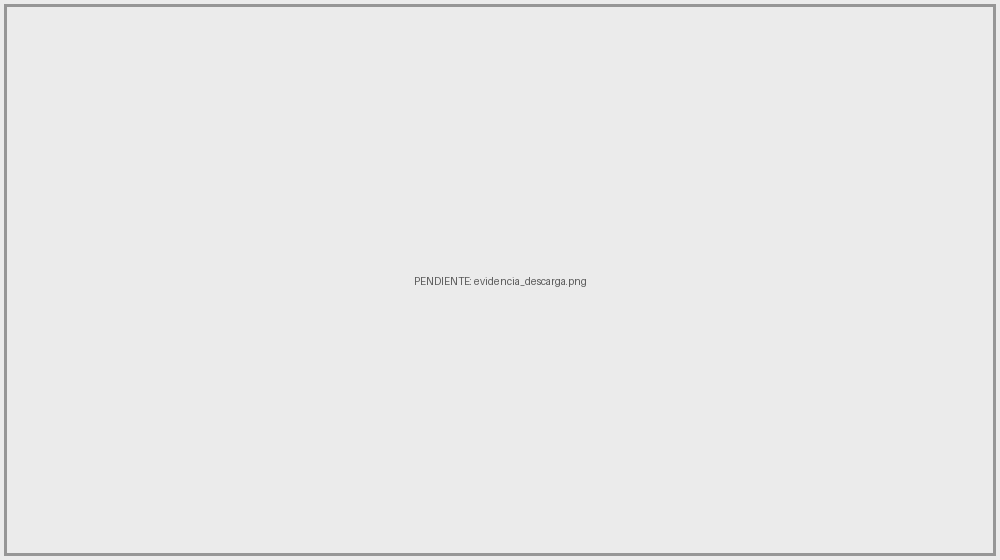
\includegraphics[width=0.95\linewidth]{evidencia_descarga.png}
	\caption{Contenido descargado del minisitio, dentro de \texttt{sitio/}}
	\label{img:descarga}
\end{figure}

\subsection{\color{colorESCOM}{Los Dockerfiles}}

Se escribieron dos \texttt{Dockerfile} distintos que comparten el mismo contenido (\texttt{sitio/}) pero cada uno lo sirve con un servidor web diferente. La única diferencia real entre ambos es la carpeta de destino del \texttt{COPY}, que depende de dónde cada imagen oficial espera su \emph{document root}.

\begin{lstlisting}[language=bash, caption={Dockerfile.apache: imagen basada en httpd}]
FROM httpd:2.4-alpine

COPY sitio/ /usr/local/apache2/htdocs/

EXPOSE 80
\end{lstlisting}

\begin{itemize}
	\item \texttt{FROM httpd:2.4-alpine} parte de la imagen oficial de Apache HTTP Server 2.4 sobre Alpine Linux, una distribución mínima que mantiene la imagen ligera \cite{httpd-docker}.
	\item \texttt{COPY sitio/ /usr/local/apache2/htdocs/} copia el sitio dentro del \emph{document root} por defecto de esa imagen.
	\item \texttt{EXPOSE 80} documenta que el proceso dentro del contenedor escucha en el puerto 80; es informativo y no publica el puerto por sí solo, eso lo hace \texttt{-p} en \texttt{docker run}.
\end{itemize}

\begin{lstlisting}[language=bash, caption={Dockerfile.nginx: imagen basada en nginx}]
FROM nginx:alpine

COPY sitio/ /usr/share/nginx/html/

EXPOSE 80
\end{lstlisting}

\begin{itemize}
	\item \texttt{FROM nginx:alpine} parte de la imagen oficial de Nginx sobre Alpine \cite{nginx-docker}.
	\item \texttt{COPY sitio/ /usr/share/nginx/html/} copia el mismo sitio, ahora en el \emph{document root} por defecto de Nginx, distinto al de Apache y la única razón por la que se necesitan dos \texttt{Dockerfile} en vez de uno solo.
	\item \texttt{EXPOSE 80} tiene el mismo papel documental que en la imagen de Apache.
\end{itemize}

\subsection{\color{colorESCOM}{Construcción de las imágenes (\texttt{docker build})}}

Ambas imágenes se construyen desde la misma carpeta de contexto (esta práctica), seleccionando el \texttt{Dockerfile} correspondiente con la bandera \texttt{-f} y etiquetándolas (\texttt{-t}) con un nombre memorable:

\begin{lstlisting}[language=bash, caption={Construcción de las dos imágenes}]
docker build -f Dockerfile.apache -t nuevoingreso-apache .
docker build -f Dockerfile.nginx  -t nuevoingreso-nginx  .
\end{lstlisting}

En ambos casos Docker procesa el \texttt{Dockerfile} instrucción por instrucción, descarga la imagen base si no está en caché local, y agrega una capa por cada instrucción hasta terminar con la imagen etiquetada y lista para ejecutarse.

\begin{figure}[H]
	\centering
	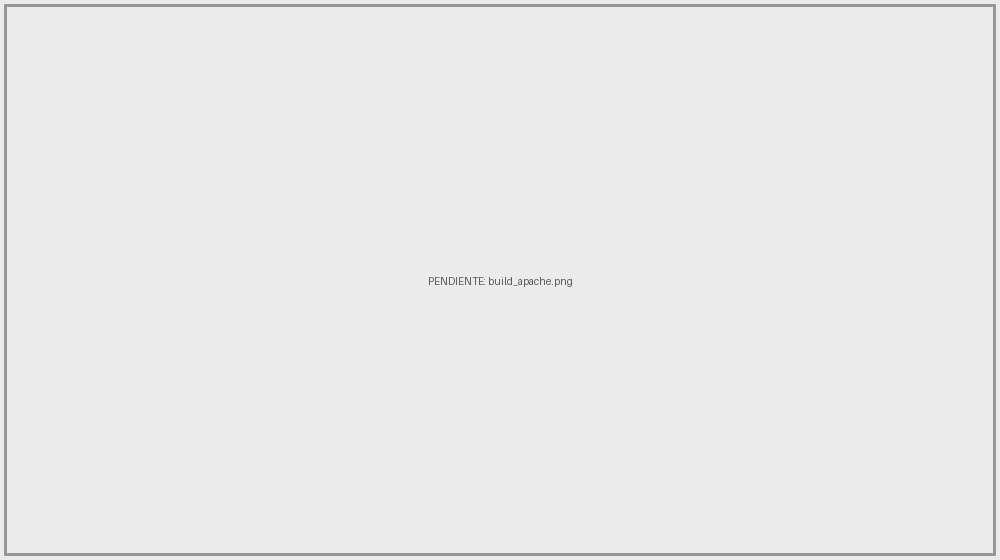
\includegraphics[width=0.95\linewidth]{build_apache.png}
	\caption{\texttt{docker build} de la imagen basada en Apache}
	\label{img:build-apache}
\end{figure}

\begin{figure}[H]
	\centering
	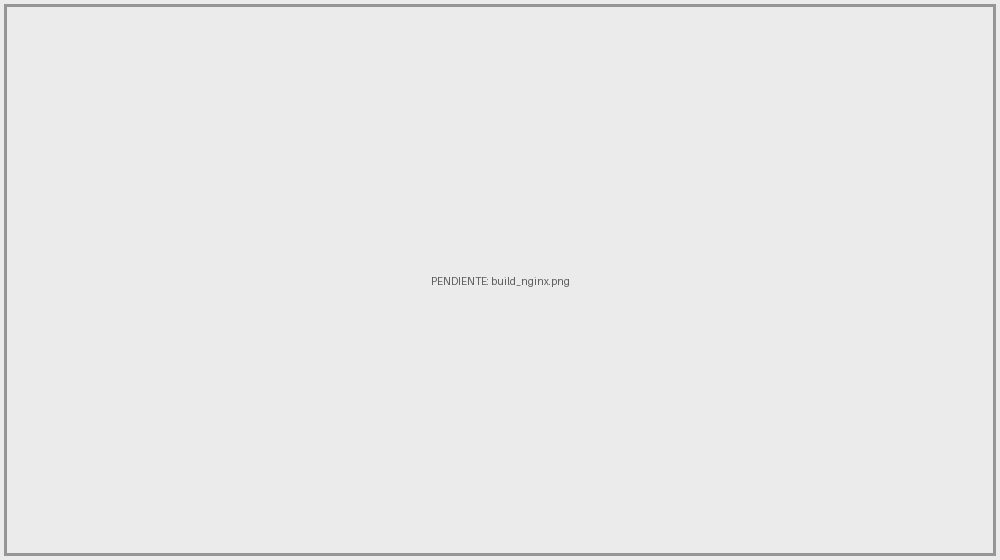
\includegraphics[width=0.95\linewidth]{build_nginx.png}
	\caption{\texttt{docker build} de la imagen basada en Nginx}
	\label{img:build-nginx}
\end{figure}

\subsection{\color{colorESCOM}{Ejecución de los contenedores (\texttt{docker run})}}

Con las dos imágenes ya construidas, se levanta un contenedor de cada una, publicando puertos distintos del anfitrión hacia el puerto 80 interno de cada contenedor para que ambos puedan convivir sin chocar:

\begin{lstlisting}[language=bash, caption={Ejecución de ambos contenedores}]
docker run --name nuevoingreso-apache -d -p 8080:80 nuevoingreso-apache
docker run --name nuevoingreso-nginx  -d -p 8081:80 nuevoingreso-nginx

docker ps
\end{lstlisting}

La bandera \texttt{-d} corre el contenedor en segundo plano, \texttt{--name} le da un nombre legible en vez del identificador aleatorio por defecto, y \texttt{-p 8080:80}/\texttt{-p 8081:80} son los mapeos de puerto descritos en la sección de conceptos teóricos: el 8080 y el 8081 del anfitrión quedan enlazados al 80 de cada contenedor respectivamente.

\begin{figure}[H]
	\centering
	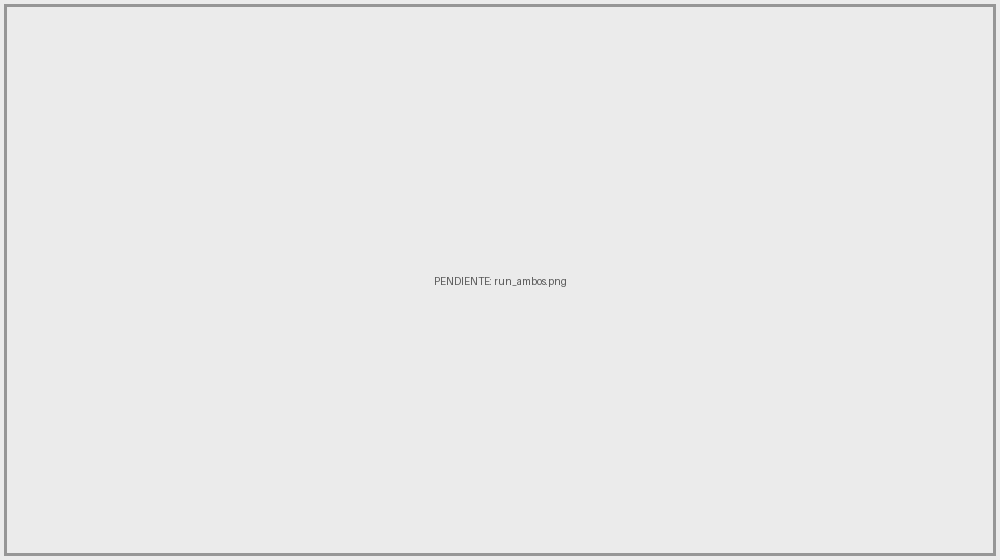
\includegraphics[width=0.95\linewidth]{run_ambos.png}
	\caption{Ambos contenedores corriendo simultáneamente (\texttt{docker ps})}
	\label{img:run}
\end{figure}

%################################################
\section{\color{colorIPN}{Resultados}}

Con los dos contenedores arriba, el mismo minisitio responde en dos puertos distintos del anfitrión servido por dos motores distintos:

\begin{table}[H]
	\centering
	\begin{tabular}{@{}llll@{}}
		\toprule
		Servidor & Imagen base & Document root & URL \\
		\midrule
		Apache httpd & \texttt{httpd:2.4-alpine} & \texttt{/usr/local/apache2/htdocs/} & \texttt{http://localhost:8080} \\
		Nginx        & \texttt{nginx:alpine}     & \texttt{/usr/share/nginx/html/}    & \texttt{http://localhost:8081} \\
		\bottomrule
	\end{tabular}
	\caption{Las dos instancias del mismo sitio, una por servidor}
	\label{tab:resultados}
\end{table}

\begin{figure}[H]
	\centering
	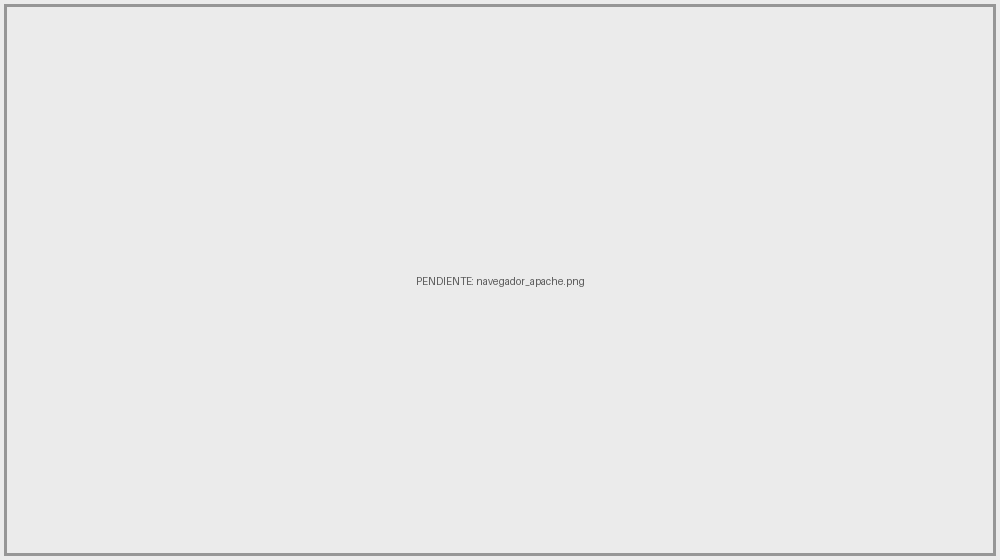
\includegraphics[width=0.95\linewidth]{navegador_apache.png}
	\caption{Minisitio funcionando en \texttt{http://localhost:8080}, servido por Apache}
	\label{img:nav-apache}
\end{figure}

\begin{figure}[H]
	\centering
	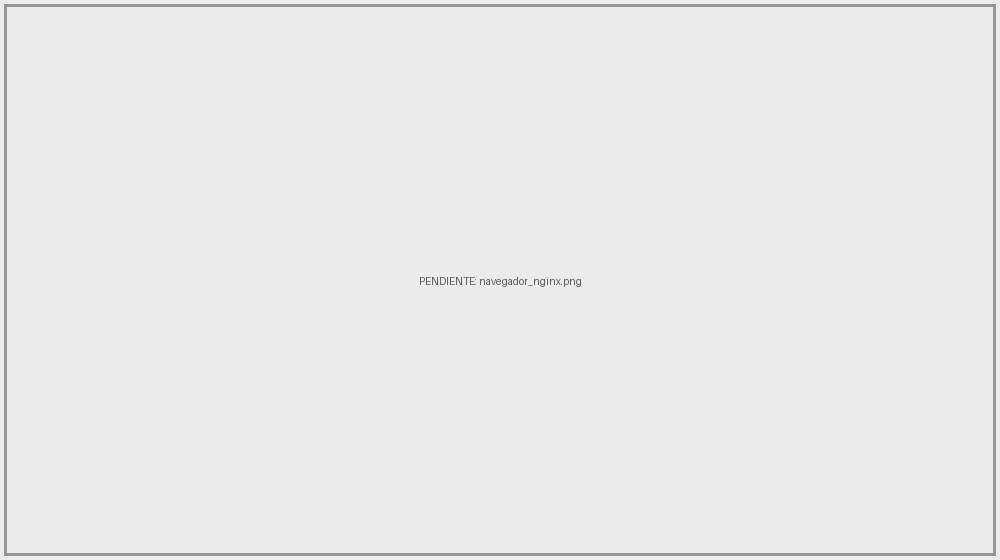
\includegraphics[width=0.95\linewidth]{navegador_nginx.png}
	\caption{Minisitio funcionando en \texttt{http://localhost:8081}, servido por Nginx}
	\label{img:nav-nginx}
\end{figure}

Las dos capturas muestran el mismo contenido con la misma apariencia, lo cual confirma que el sitio no depende de ninguna característica propia de un servidor en particular: es HTML y CSS estático, así que a cualquiera de los dos motores les basta con entregar los archivos tal cual.

%################################################
\section{\color{colorIPN}{Conclusiones}}

Apache y Nginx no coinciden en dónde esperan encontrar los archivos a servir (\texttt{/usr/local/apache2/htdocs/} contra \texttt{/usr/share/nginx/html/}), y esa diferencia fue la dificultad real de la práctica: copiar el mismo \texttt{sitio/} a la ruta equivocada produce la página por defecto del servidor en vez del minisitio. Confirmar el \emph{document root} de cada imagen oficial antes de escribir el \texttt{COPY} evitó ese tropiezo. La segunda dificultad, más práctica que conceptual, fue mantener los puertos publicados sin choques: al correr ambos contenedores sobre el mismo anfitrión, publicar los dos en el mismo puerto externo (por ejemplo, 8080 para los dos) hace que el segundo \texttt{docker run} falle porque el puerto ya está tomado, de ahí que cada contenedor use un puerto distinto del anfitrión aunque los dos escuchen internamente en el 80.

Más allá de esos dos detalles, el ejercicio deja clara la separación de responsabilidades que ofrece Docker: la misma carpeta de contenido, sin modificar una sola línea, se sirve igual de bien desde dos servidores completamente distintos con solo cambiar el \texttt{Dockerfile} que la empaqueta. Esa portabilidad (contenido separado del servidor que lo entrega, y servidor separado del sistema operativo que lo hospeda) es exactamente el problema que las arquitecturas contenedorizadas de la Unidad V de esta materia dan por resuelto, y que aquí se comprobó con un caso mínimo.

%################################################
\pagebreak
\printbibliography[heading=none]

\end{document}
